\documentclass[11pt, letterpaper]{article}

\usepackage[margin=1in, headheight=15pt]{geometry}
\usepackage{graphicx}
\usepackage{hyperref}
\usepackage{xcolor}
\usepackage{listings}
\usepackage{booktabs}
\usepackage{array}
\usepackage{parskip}
\usepackage{titlesec}
\usepackage{fancyhdr}
\usepackage{enumitem}
\usepackage{microtype}
\usepackage{float}

\definecolor{codegreen}{rgb}{0.0, 0.5, 0.0}
\definecolor{codegray}{rgb}{0.5, 0.5, 0.5}
\definecolor{codepurple}{rgb}{0.4, 0.0, 0.6}
\definecolor{codeblue}{rgb}{0.0, 0.2, 0.6}
\definecolor{backcolour}{rgb}{0.97, 0.97, 0.97}
\definecolor{linkblue}{rgb}{0.1, 0.2, 0.7}

\hypersetup{colorlinks=true, linkcolor=linkblue, urlcolor=linkblue}

\lstdefinestyle{code}{
    backgroundcolor=\color{backcolour},
    commentstyle=\color{codegreen}\itshape,
    keywordstyle=\color{codeblue}\bfseries,
    numberstyle=\tiny\color{codegray},
    stringstyle=\color{codepurple},
    basicstyle=\ttfamily\small,
    breaklines=true,
    numbers=left,
    numbersep=8pt,
    frame=single,
    framesep=4pt,
    rulecolor=\color{gray!40},
    showstringspaces=false,
    tabsize=4,
}
\lstset{style=code}

\titleformat{\section}{\large\bfseries}{}{0em}{}[\titlerule]
\titleformat{\subsection}{\normalsize\bfseries}{}{0em}{}

\pagestyle{fancy}
\fancyhf{}
\rhead{\small SSH Auto-Ban System}
\lhead{\small CS 6324 --- Network Security}
\cfoot{\thepage}
\renewcommand{\headrulewidth}{0.4pt}

\begin{document}

% --- Title ---
\begin{titlepage}
    \centering
    \vspace*{2.5cm}
    {\huge\bfseries Detecting Repeated SSH Connections\\[0.4em]
    via IP Address Reputation\par}
    \vspace{2cm}

    \begin{tabular}{ll}
        \textbf{Supakjeera Thanapaisal} & \texttt{SXT240029} \\[0.4em]
        \textbf{Timothy Sweet}          & \texttt{TRS200004} \\[0.4em]
        \textbf{Sherry Cherniavsky}     & \texttt{SXC210068} \\
    \end{tabular}

    \vspace{1.5cm}
    \textbf{GitHub:} \small\url{https://github.com/nthanapaisal/ssh-auth-attempt-reputation-based-ban}\\[0.6em]
    \textbf{Demo:} \small\url{https://drive.google.com/file/d/1AE0Qgp4-mZ4TQUMjSl7HzM1Cr6tSwqMc/view}

    \vfill
    {\normalsize April 2026}
\end{titlepage}

\tableofcontents
\newpage

% --- 1. Introduction ---
\section{Introduction}

A lightweight security system that detects and blocks repeated SSH authentication attempts on a Linux VPS using Autonomous System (AS) reputation. The system monitors authentication logs, evaluates attacker reputation via AbuseIPDB, and dynamically updates \texttt{nftables} firewall rules to block malicious connections.

The key advantage over tools like Fail2ban is that banning decisions are informed by \textit{global} reputation data rather than only locally-observed failures. An IP already known to be malicious can be blocked on its very first attempt against the local server, without waiting for a failure threshold to be crossed. A local SQLite cache keeps API usage efficient --- the external service is only consulted when the information would genuinely be new.

Three components cooperate to achieve this: a \textbf{log listener service} that tails the systemd journal for SSH failure events, a \textbf{reputation service} that decides whether a given IP should be blocked, and an \textbf{nftables firewall configuration} that enforces those decisions at the kernel level.

% --- 2. Background and Motivation ---
\section{Background and Motivation}

\subsection{The Problem}

SSH servers exposed to the internet are constant targets for automated brute-force attacks. Even failed attempts flood logs, consume CPU handling rejected handshakes, and make it harder to spot legitimate anomalies. At high enough volumes, this traffic can degrade SSH availability for real users.

\subsection{Existing Defenses}

Tools like Fail2ban and DenyHosts ban IPs after a locally-observed failure threshold is crossed. They are purely reactive --- an IP that has been attacking other servers for months still gets several free attempts locally before any ban is applied. Static blocklists offer proactive blocking but require constant manual maintenance and go stale quickly.

SSH servers can and should be configured with strong authentication --- ideally key-based only, with password auth disabled --- to prevent any attempt from succeeding. However, blocking repeated failed attempts at the firewall level is still valuable independent of authentication strength.

\subsection{Threat Model}

The threat modeled here is \textbf{denial-of-service via SSH flooding}: high volumes of repeated, failed authentication attempts. Successful attacker login is out of scope --- that is prevented by key-based authentication. Two concrete harms motivate blocking this traffic even when it cannot succeed:

\begin{enumerate}[leftmargin=2em, itemsep=2pt]
    \item Repeated failed attempts clog the system log, making it harder to find real entries and troubleshoot SSH-related issues.
    \item At sufficient volume, the connection overhead can consume enough resources that SSH becomes slow or difficult to reach for legitimate users.
\end{enumerate}

By blocking traffic from known-bad IPs at the kernel level, the system prevents \texttt{sshd} from ever processing those connections.

% --- 3. Design ---
\section{Design}

\subsection{Architecture}

\begin{figure}[H]
    \centering
    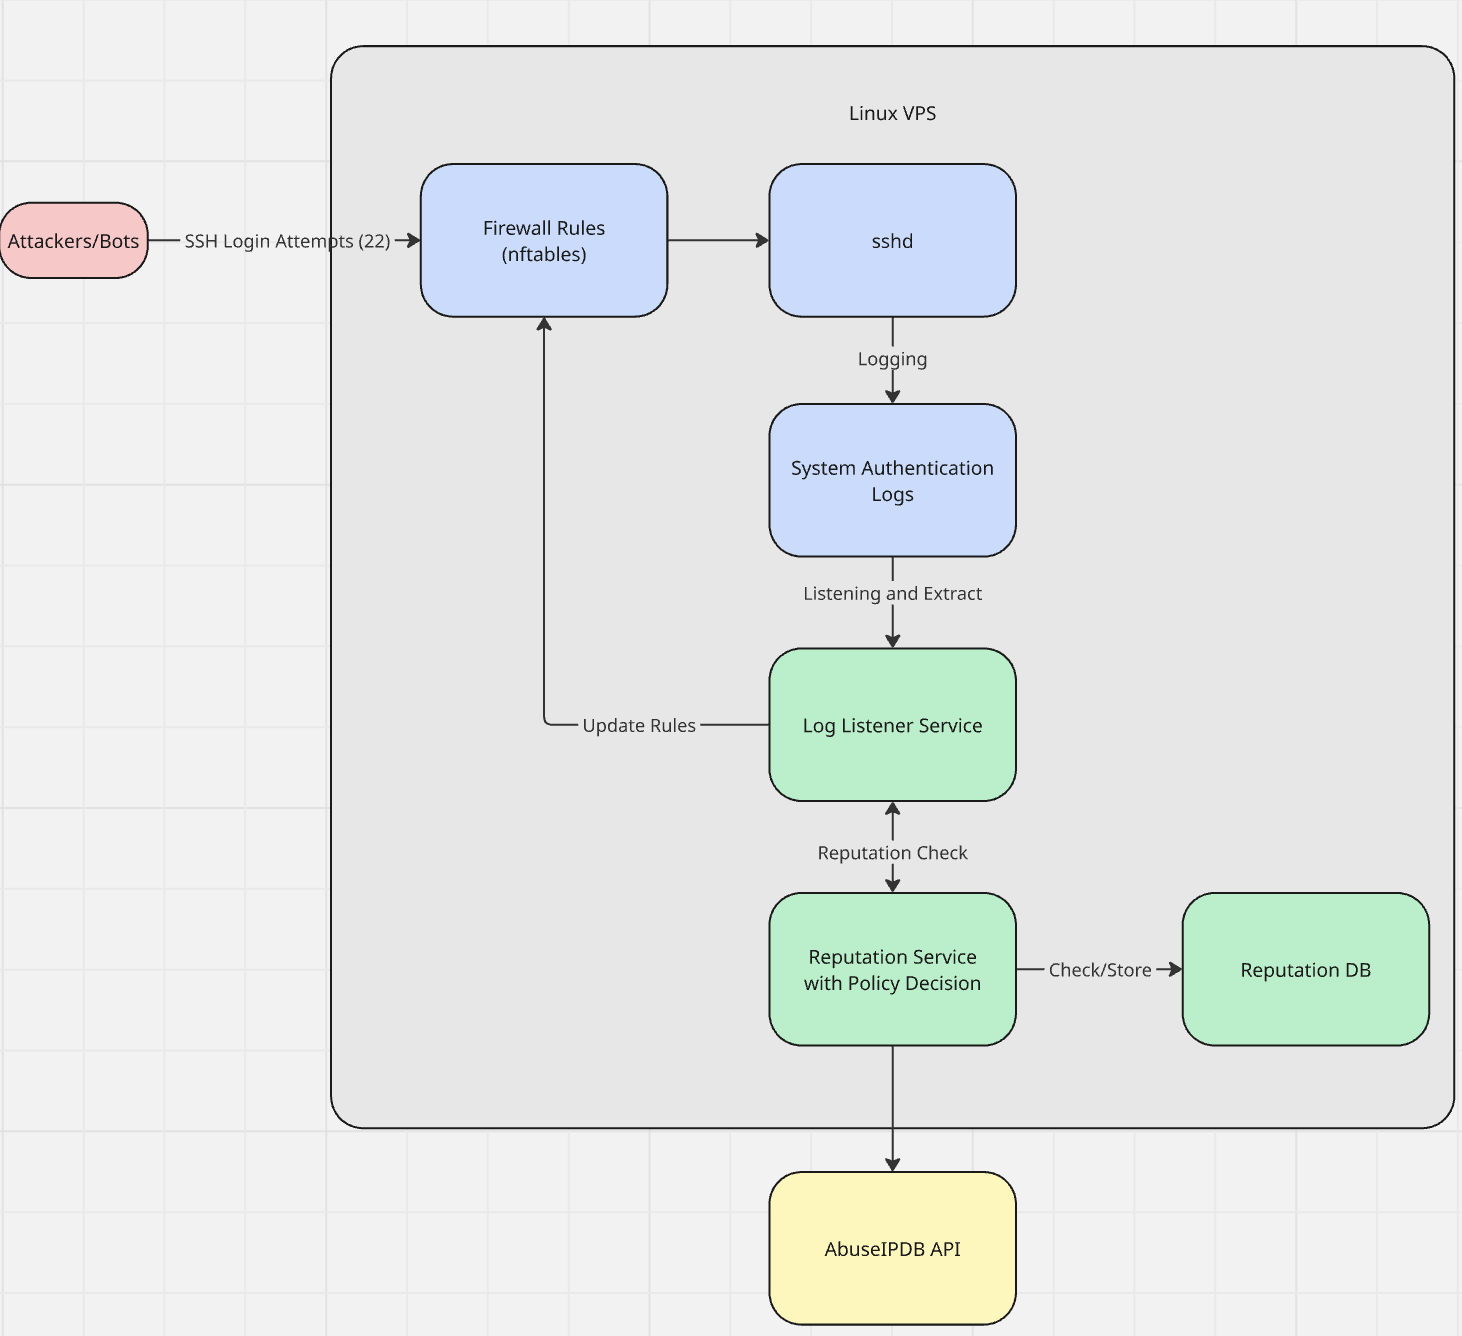
\includegraphics[width=0.82\textwidth]{architecture_diagram.png}
    \caption{High-level architecture diagram.}
\end{figure}

Incoming SSH attempts pass through \texttt{nftables}. If not already banned, \texttt{sshd} processes the attempt and writes a log entry to the systemd journal. The listener watches for failure log entries, extracts the source IP, and passes it to the reputation service. The reputation service checks a local SQLite cache, calls AbuseIPDB if needed, and returns a block-or-allow decision. A block decision causes the listener to insert the IP into an \texttt{nftables} set with a 12-hour expiration.

\subsection{Components}

\begin{table}[H]
    \centering
    \begin{tabular}{>{\bfseries\ttfamily}p{4.8cm} p{9.2cm}}
        \toprule
        File & Responsibility \\
        \midrule
        listener\_service.py &
            Monitors \texttt{ssh.service} journal entries in real time. Extracts source IPs from failure log messages and invokes the reputation service. \\[0.4em]
        reputation\_service.py &
            Validates IPs, checks the SQLite cache, queries AbuseIPDB when needed, and returns a block decision. \\[0.4em]
        ssh\_auto\_ban-default.nft &
            Defines \texttt{nftables} sets for banned IPv4/IPv6 addresses with a drop rule on the input chain. \\
        \bottomrule
    \end{tabular}
\end{table}

% --- 4. Component Design ---
\section{Component Design}

\subsection{Listener Service (\texttt{listener\_service.py})}

On startup, the listener loads \texttt{ssh\_auto\_ban-default.nft} via \texttt{nft -f} to initialize the firewall sets, then opens a \texttt{systemd.journal.Reader} filtered to \texttt{ssh.service}. It seeks to the journal tail (ignoring historical entries) and registers the file descriptor with \texttt{select.poll()}, blocking until new entries arrive.

Each new entry's \texttt{MESSAGE} field is matched against four patterns:

\begin{itemize}[leftmargin=1.5em, itemsep=2pt]
    \item \texttt{Failed password for [invalid user] <user> from <ip>} --- password auth failure.
    \item \texttt{Unable to negotiate with <ip>} --- cipher/key-exchange mismatch; typical of automated scanners probing with non-standard parameters.
    \item \texttt{banner exchange: Connection from <ip>} --- low-level protocol failure before authentication; characteristic of scan tools.
    \item \texttt{Invalid user <user> from <ip>} / \texttt{Connection closed by authenticating user} --- only matched when \texttt{SSH\_HAS\_PASS\_AUTH\_DISABLED = True}. When password auth is enabled, these events overlap with the failed password pattern and would double-count the same connection.
\end{itemize}

If a match is found, the IP is passed to \texttt{handle\_bad\_ip}, which calls the reputation service. On a block decision, \texttt{ban\_bad\_ip} determines IPv4 vs.\ IPv6 using Python's \texttt{ipaddress} module and inserts the address into the appropriate \texttt{nftables} set:
\vspace{6pt}
\begin{lstlisting}[language=bash]
nft add element inet ssh_auto_bans <set> { <ip> timeout 12h }
\end{lstlisting}

The 12-hour timeout is handled natively by the kernel --- no external cleanup process is needed.

\subsection{Reputation Service (\texttt{reputation\_service.py})}

\subsubsection*{IP Validation}

Before any cache or API call, the IP is validated with \texttt{ipaddress.ip\_address()}. Non-global addresses (private, loopback, link-local) immediately return \texttt{False}. This prevents the system from acting on log messages that reference internal addresses and ensures nothing private is sent to the external API.

\subsubsection*{Caching and Decision Logic}

AbuseIPDB provides an \textit{abuse confidence score} (0--100) reflecting community-reported malicious activity. Scores above 80 result in a block. Rather than querying the API on every connection, the service uses a tiered cache to decide when a fresh lookup is warranted:

\begin{enumerate}[leftmargin=2em, itemsep=2pt]
    \item \textbf{Not in DB} --- query AbuseIPDB, store result, return decision.
    \item \textbf{In DB, already blocked} --- return \texttt{True} immediately; increment counter.
    \item \textbf{In DB, not blocked, cache fresh} ($\leq$1 hour since last check) --- return \texttt{False}; increment counter.
    \item \textbf{In DB, not blocked, cache expired, count $\leq$ 20} --- return \texttt{False}; increment counter. The IP is not appearing frequently enough for a fresh lookup to matter.
    \item \textbf{In DB, not blocked, cache expired, count $>$ 20} --- the IP is persisting despite not being blocked. Query AbuseIPDB for a fresh score, update DB, return new decision.
\end{enumerate}

\subsubsection*{Database Schema}
\vspace{6pt}
\begin{lstlisting}[language=SQL]
CREATE TABLE IF NOT EXISTS ip_rep_db (
    ip           TEXT    PRIMARY KEY,
    score        INTEGER NOT NULL,
    checked_at   INTEGER NOT NULL,  -- Unix timestamp of last API call
    num_connects INTEGER NOT NULL,  -- connections since last API call
    is_blocked   INTEGER NOT NULL
);
\end{lstlisting}

\subsection{nftables Configuration (\texttt{ssh\_auto\_ban-default.nft})}

Defines an \texttt{inet} table (covering both IPv4 and IPv6) with two sets: \texttt{banned\_v4} and \texttt{banned\_v6}. Both use \texttt{flags timeout} so that individual entries expire automatically. A single input chain with default \texttt{accept} policy drops and logs any packet whose source address appears in either set.
\vspace{6pt}
\begin{lstlisting}[language=bash]
table inet ssh_auto_bans {
    set banned_v4 { type ipv4_addr; flags timeout }
    set banned_v6 { type ipv6_addr; flags timeout }

    chain input {
        type filter hook input priority 0; policy accept;
        ip  saddr @banned_v4 log prefix "SSH autoban: " drop
        ip6 saddr @banned_v6 log prefix "SSH autoban: " drop
    }
}
\end{lstlisting}

% --- 5. Program Flow Summary ---
\newpage
\section{Program Flow Summary}

\begin{enumerate}[leftmargin=2em, itemsep=2pt]
    \item Monitors \texttt{ssh.service} logs through \texttt{systemd.journal}.
    \item Extracts source IPs from failed or suspicious SSH log messages.
    \item Sends the IP to the reputation service.
    \item Validates that the IP is a real global/public address.
    \item Checks the local SQLite cache.
    \item Calls AbuseIPDB only if:
        \begin{enumerate}[label=\arabic{enumi}.\arabic*, leftmargin=1.5em, itemsep=1pt]
            \item the IP is not in cache, or
            \item the cache is expired and the IP has exceeded the connection threshold.
        \end{enumerate}
    \item Stores or updates the IP record in SQLite.
    \item Returns whether the IP should be blocked.
    \item If blocked, adds the IP to an \texttt{nftables} ban set with a 12-hour timeout.
\end{enumerate}

The goal is to reduce repeated malicious SSH connection attempts by using IP reputation data together with a local cache, rather than calling the external API on every connection.

% --- 6. Evaluation ---
\section{Evaluation}

\subsection{Experimental Setup}
The test was conducted on a cloud VPS with port 22 (\texttt{sshd}) exposed to the internet. It was measured over a period from \texttt{2026-04-28 15:33:33 UTC} to \texttt{2026-04-30 08:36:55 UTC} (approximately 2 days and 5 hours). During this time:
\begin{itemize}
    \item Existing \texttt{fail2ban} protections were disabled.
    \item \texttt{sshd} password authentication was enabled.
    \item No legitimate login attempts were made.
\end{itemize}

\subsection{Observed Traffic}
\begin{table}[h]
\centering
\begin{tabular}{lcc}
\hline
\textbf{Metric} & \textbf{Count} & \textbf{Unique IPs} \\
\hline
Connections reaching \texttt{sshd} & 3,379 & 203 \\
Connections blocked by firewall & 20,609 & 163 \\
\hline
Total observed attempts & 23,988 & 203 \\
\hline
\end{tabular}
\caption{Summary of observed SSH connection attempts}
\end{table}

\subsection{Effectiveness of Filtering}
From the observed data:
\begin{itemize}
    \item Only \textbf{16.4\%} of total connection attempts reached \texttt{sshd}.
    \item The firewall blocked \textbf{83.6\%} of all attempts before they reached the service.
    \item \textbf{80.2\%} of unique IP addresses were blocked after their first attempt, preventing repeated probing.
\end{itemize}

\subsection{Discussion}
As we intended, the firewall rules eliminate the vast majority of connection attempts, with 80.2\% of all IPs that attempt to connect to us being blocked on the very first try, and 83.6\% of total connections never reach \texttt{sshd} at all. This indicates that utilizing crowd-sourced IP reputation info is a useful layer of defense to reduce connection attempts and load on \texttt{sshd}, in addition to further layers such as traditional fail2ban and of course, strong authentication.


% --- 7. Installation ---
\section{Installation}


\textbf{Prerequisites:} Python 3.8+, \texttt{nftables}, \texttt{systemd}, and an AbuseIPDB API key (\url{https://www.abuseipdb.com/}).
\vspace{6pt}
\begin{lstlisting}[language=bash]
# Set environment variables
export ABUSEIPDB_API_KEY="your_key_here"
export REPUTATION_DB_PATH="path/to/reputation.sqlite"

# Clone and install
git clone https://github.com/nthanapaisal/ssh-auth-attempt-reputation-based-ban.git
cd ssh-auth-attempt-reputation-based-ban
pip install -r requirements.txt

# Run (requires root for nftables)
sudo python listener_service.py
\end{lstlisting}

\end{document}
